\section{Benchmark}

Pour évaluer notre implémentation nous avons réalisé un petit benchmark qui se charge de simuler un
scénario basique.

\subsection{Scénario}

Nous voulons tester un scénario comparable à celui présenté dans la partie \textbf{4.1 Monocœur}.
Un thread parent prend un mutex et lance l'exécution de N threads enfants se bloquant sur son mutex.
Une fois les enfants lancés, le parent exécute son calcul.
X autres threads s'exécutent en parallèle du thread parent et effectue leur calcul.
Le programme s'arrête brutalement quand le parent a fini l'exécution de son calcul.

\noindent \textbf{Calcul des threads:} 
Calcul du déterminent d'une matrice 11x11.

\noindent \textbf{Résultat attendu:}
Les N threads enfants doivent augmenter la priorité du thread parent de N. Le thread parent doit donc voir son temps d'exécution significativement réduit en fonction de N et finir avant les X threads parallèles.

\noindent \textbf{Environnement de test:}
Machine virtuelle avec 1 cœur.

\subsection{Résultat}

Dans un premier temps nous avons mesuré le temps nécessaire au thread parent pour exécuter son calcul
sans thread parallèle, qui serait concurrent, et sans enfant.
Ce temps d'exécution est noté baseline est correspond à 1,8s.

Nous avons fait évoluer le nombre de threads enfants de 0 à 50 avec 100 threads parallèles. 
Les résultats présentés dans la Figure \ref{fig:result} nous montre que le temps d'exécution
du thread parent tend vers la baseline quand sa priorité augmente dû aux threads enfants qu'il bloque.
Ce qui est le résultat escompté. 

\begin{figure}[h!]
	\centering
	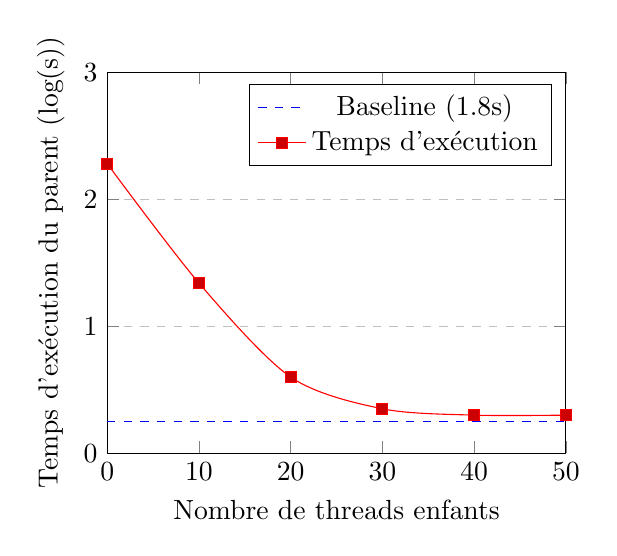
\begin{tikzpicture}
	\begin{axis}[
	xlabel={Nombre de threads enfants},
	ylabel={Temps d'exécution du parent (log(s))},
	xmin=0, xmax=50,
	ymin=0, ymax=3,
	legend pos=north east,
	ymajorgrids=true,
	grid style=dashed,
	scale=0.85,
	]
	\addplot[color=blue, style=dashed]
	coordinates {(0,0.25)(4000,0.25)};
	\addplot+[smooth,color=red]
	coordinates {(0,2.28)(10,1.34)(20,0.6)(30,0.35)(40,0.3)(50,0.3)};
	\legend{Baseline (1.8s), Temps d'exécution}
	\end{axis}
	\end{tikzpicture}
	\caption{Temps d'exécution avec 100 threads parallèles}
	\label{fig:result}
\end{figure}

\newpage

En deuxième lieu nous avons fait évoluer le nombre de thread parallèle de 0 à 100 avec 50 threads enfants.

La Figure \ref{fig:with} nous montre les résultats avec notre mécanisme. On remarque que le thread parent 
reste proche de la baseline bien que le nombre de threads parallèle augmente. Les threads enfants bloqués permettent au
thread parent, par le biais de notre mécanisme, d'être toujours plus prioritaire que les threads parallèle, quelque soit leur nombre.

La Figure \ref{fig:without} nous montre les résultats sans notre mécanisme. Le thread parent voit son temps d'exécution
croître quand le nombre de threads parallèle augmente, car sans la modification de priorité induite par les threads
enfants bloqués, le thread parent n'est pas plus prioritaire que les threads parallèles.

Notre implémentation a ajouté un overhead sur le kernel. La Figure \ref{fig:overhead} montre l'impact de
l'overhead sur le temps d'exécution côté kernel. Ce ralentissement peut notamment être dû à l'utilisation de
spinlock lors de la manipulation des listes, mais aussi les calculs d'héritages. Cependant la différence reste
faible et minime face au gain de temps induit par le mécanisme.


\begin{figure}
	\centering
	\begin{minipage}{0.45\textwidth}
		\centering
		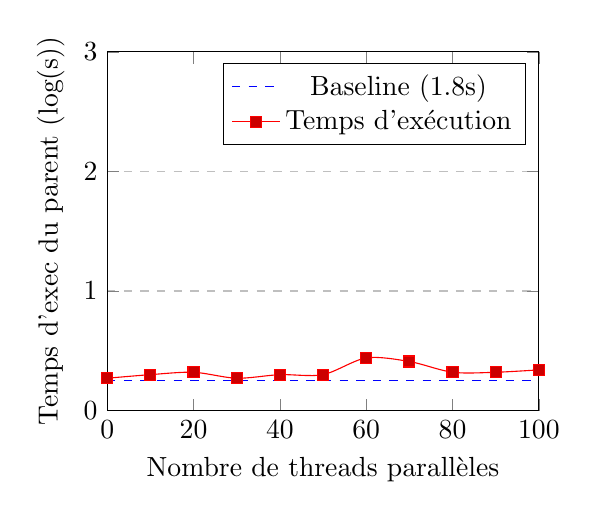
\begin{tikzpicture}
		\begin{axis}[
		xlabel={Nombre de threads parallèles},
		ylabel={Temps d'exec du parent (log(s))},
		xmin=0, xmax=100,
		ymin=0, ymax=3,
		legend pos=north east,
		ymajorgrids=true,
		grid style=dashed,
		scale=0.80,
		]
		
		\addplot[color=blue, style=dashed]
		coordinates {(0,0.25)(4000,0.25)};
		\addplot+[smooth,color=red]
		coordinates {(0,0.27)(10,0.3)(20,0.32)(30,0.27)(40,0.3)(50,0.3)
			(60,0.44)(70,0.41)(80,0.32)(90,0.32)(100,0.34)};
		\legend{Baseline (1.8s), Temps d'exécution}
		\end{axis}
		\end{tikzpicture}
		\caption{\textbf{avec} l'implémentation futex\_state}
		\label{fig:with}
	\end{minipage}\hfill
	\begin{minipage}{0.45\textwidth}
		\centering
		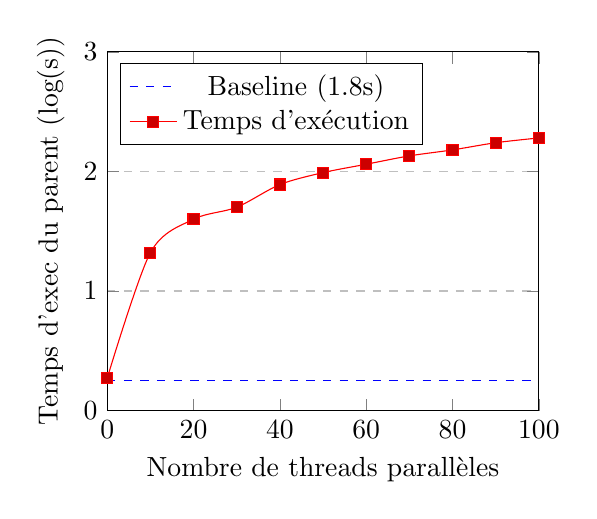
\begin{tikzpicture}
		\begin{axis}[
		xlabel={Nombre de threads parallèles},
		ylabel={Temps d'exec du parent (log(s))},
		xmin=0, xmax=100,
		ymin=0, ymax=3,
		legend pos=north west,
		ymajorgrids=true,
		grid style=dashed,
		scale=0.80,
		]
		\addplot[color=blue, style=dashed]
		coordinates {(0,0.25)(4000,0.25)};
		\addplot+[smooth,color=red]
		coordinates {(0,0.27)(10,1.32)(20,1.6)(30,1.7)(40,1.89)(50,1.99)
			(60,2.06)(70,2.13)(80,2.18)(90,2.24)(100,2.28)};
		\legend{Baseline (1.8s), Temps d'exécution}
		\end{axis}
		\end{tikzpicture}
		\caption{\textbf{sans} l'implémentation futex\_state}
		\label{fig:without}
	\end{minipage}
\end{figure}


\begin{figure}[h!]
	\centering
	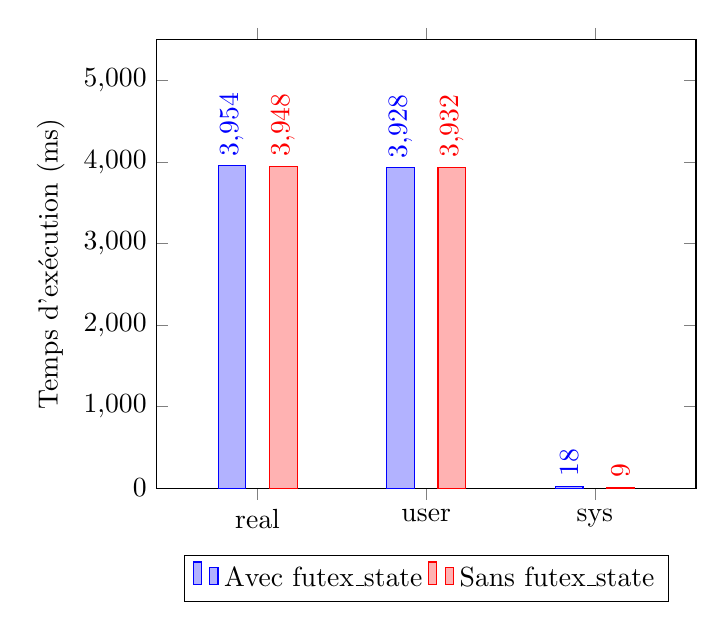
\begin{tikzpicture}
	\begin{axis}[
	ybar=.3cm,
	enlarge x limits={0.30},
	ymin=0, ymax=5500,
	legend style={at={(0.5,-0.15)},
		anchor=north,legend columns=-1},
	ylabel={Temps d'exécution (ms)},
	symbolic x coords={real,user,sys},
	xtick=data,
	nodes near coords = \rotatebox{90}{{\pgfmathprintnumber[fixed zerofill, precision=0]{\pgfplotspointmeta}}},
	nodes near coords align={vertical},
	]
	\addplot coordinates {(real,3954) (user,3928) (sys,18)};
	\addplot coordinates {(real,3948) (user,3932) (sys,9)};
	\legend{Avec futex\_state, Sans futex\_state}
	\end{axis}
	\end{tikzpicture}
	\caption{Ralentissement dû à l'overhead de notre implémentation}
	\label{fig:overhead}
\end{figure}
